	
	On peut dresser un arbre pondéré :
	\begin{center}
	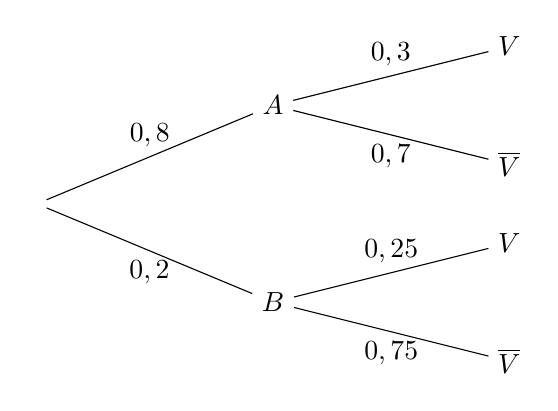
\begin{tikzpicture}
		[level 1/.style={level distance=3cm,
			sibling distance=2.5cm},
		level 2/.style={level distance=3cm,
			sibling distance=1.5cm}
		]
		\node {} [grow'=right]
		child {node {$A$}
			child {node {$V$}
				edge from parent node[above] {$0,3$}
			}
			child {node {$\overline V$}
				edge from parent node[below] {$0,7$}
			}
			edge from parent node[above] {$0,8$}
		}
		child {node {$B$}
			child {node {$V$}
				edge from parent node[above] {$0,25$}
			}
			child {node {$\overline V$}
				edge from parent node[below] {$0,75$}
			}
			edge from parent node[below] {$0,2$}
		}
	
		;
	\end{tikzpicture}
\end{center}


	
	\subsection*{1.}
	
	\(P_B(V) = 0,75\) signifie que la probabilité de perdre contre le monstre B est égale à 0,75.
	
	\subsection*{2.}
	
	On a \(P(B \cap V) = P(B) \times P_B(V) = 0,2 \times 0,25 = 0,05 = \dfrac{1}{20}\).
	
	\subsection*{3.}
	
	On a de même : \(P(A \cap V) = P(A) \times P_A(V) = 0,8 \times 0,3 = 0,24 = \dfrac{24}{100}\).
	
	D'après la loi des probabilités totales :
	\[
	P(V) = P(A \cap V) + P(B \cap V) = 0,24 + 0,05 = 0,29.
	\]
	
	\subsection*{4.}
	
	Il faut trouver \(P_V(B)\) :
	\[
	P_V(B) = \dfrac{P(V \cap B)}{P(V)} = \dfrac{P(B \cap V)}{P(V)} = \dfrac{0,05}{0,29} = \dfrac{5}{29} \approx 0,172.
	\]
	
